\documentclass[aps,pra,notitlepage,amsmath,amssymb,letterpaper,12pt]{revtex4-1}
\usepackage{amsthm}
\usepackage{graphicx}

\documentclass[12pt]{amsart}
\usepackage[english]{babel}
\parindent=0.pt
\usepackage{amsmath}
\usepackage{graphicx}
\usepackage{subcaption}
\graphicspath{ {} }

\usepackage{amssymb}
%\usepackage{mathrsfs}
\usepackage{enumerate}
\usepackage[notcite, final, notref]{showkeys}
\renewcommand{\theequation}{\thesection.\arabic{equation}}
\newtheorem{theorem}{Theorem}[section]
\newtheorem{problem}[theorem]{Problem}
\newtheorem{lemma}[theorem]{Lemma}
\newtheorem{proposition}[theorem]{Proposition}
\newtheorem{corollary}[theorem]{Corollary}
\newtheorem{definition}[theorem]{Definition}

\theoremstyle{definition}
\newtheorem{remark}[theorem]{Remark}
\newtheorem{example}[theorem]{Example}
\newtheorem{exercise}[theorem]{Exercise}



\newcommand{\pn}{\par\noindent}
\newcommand{\CC}{\mathbb{C}}
%\newcommand{\p}{\par\noindent}
\newcommand{\oo}{\mathbb{O}}
%\newcommand{\ioo}{\mathbb{C}\mathbb{O}}
\newcommand{\ee}{{\underline e}}
\newcommand{\si}{\mathbb{S}}
\newcommand{\bn}{\bigskip\noindent}
\newcommand{\ooo}{\mathcal{O}}
\newcommand{\Span}{{\rm span}}
\newcommand{\ds}{{\displaystyle}}
\newcommand{\bs}{{\bf S}}
\newcommand{\Ci}{\mathcal{C}}
\newcommand{\Er}{\mathcal{M}}
\newcommand{\ov}{\overline}
\newcommand{\qq}{\quad}
\newcommand{\Gi}{ \mathcal{G}}
\newcommand{\bl}{ {\hbox{\vrule height 1.5mm width 2mm}}\rm  }
\newcommand{\med}{\medskip}
\newcommand{\rr}{\mathbb{R} }
\newcommand{\cc}{\mathbb{C}}
\newcommand{\hh}{\mathbb{H}}
\newcommand{\nn}{\mathbb{N}}
\newcommand{\sss}{\sigma}
\newcommand{\eee}[1]{\bf e_{#1}}
\newcommand{\ww}{\wedge}
\newcommand{\der}[2]{ \frac{ {{\partial f_{#1}}{\partial x_{#2}}}} }
\newcommand{\derr}[1]{{{\partial}\over{\partial #1}}}
\newcommand{\deri}[2]{{{\partial}/{\partial x_{#1#2}}}}
\newcommand{\pp}{\partial}
\renewcommand{\aa}{\longrightarrow}
\newcommand{\unx}{\underline{x}}
\newcommand{\uny}{\underline{y}}
\newcommand{\uns}{\underline{s}}
\newcommand{\unp}{\underline{p}}
\newcommand{\una}{\underline{a}}

\newcommand{\U}{\mathcal{U}}
\newcommand{\borel}{\mathbf{B}}
\renewcommand{\Re}{\mathrm{Re}}

\newcommand{\indi}{\mathds{1}}
\newcommand{\lap}{\mathcal{L}}

%\usepackage{xcolor}

%\usepackage{mathrsfs}
%\usepackage[dvips]{color}
\topmargin=-10mm \oddsidemargin=0mm \evensidemargin=0mm
\textheight=230mm \textwidth=160mm


\newenvironment{problem}[2][Problem]{\begin{trivlist}
\item[\hskip \labelsep {\bfseries #1}\hskip \labelsep {\bfseries #2.}]}{\end{trivlist}}
\newenvironment{solution}{\begin{proof}[Solution]}{\end{proof}}

\usepackage{listings}
\usepackage{color}

\definecolor{dkgreen}{rgb}{0,0.6,0}
\definecolor{gray}{rgb}{0.5,0.5,0.5}
\definecolor{mauve}{rgb}{0.58,0,0.82}

\lstset{frame=tb,
  language=Python,
  aboveskip=3mm,
  belowskip=3mm,
  showstringspaces=false,
  columns=flexible,
  basicstyle={\small\ttfamily},
  numbers=none,
  numberstyle=\tiny\color{gray},
  keywordstyle=\color{blue},
  commentstyle=\color{dkgreen},
  stringstyle=\color{mauve},
  breaklines=true,
  breakatwhitespace=true,
  tabsize=3
}
 
\begin{document}
\title{sumbraro.py explanation }

\author{Natanael Alpay, Conner Carnahan}
\affiliation{PHYS 220, Schmid College of Science and Technology, Chapman University}
\date{2018}
\maketitle

\tableofcontents




\maketitle
\section{Introduction}

In this file we will discuss the problem from cw12 and how we solved it. we will show the code and the problem in addition to eplanation and way of thinking.



\section{The problem} % Specify main sections this way

Consider a ball of mass $m$ with horizontal coordinate $x$ rolling in a double-well potential $V(x) = x^4/4 - x^2/2$. (This is sometimes called the "sombrero" potential. Plot it to see why, for $x\in[-1.5,1.5]$.) This potential produces a force $f_{\text{hat}}(x) = -V'(x) = -x^3 + x$ on the rolling ball. Suppose the ball also has slight friction, so experiences a drag force $f_{\text{drag}}(\dot{x}) = -\nu \dot{x}$. With these forces we thus expect the ball to roll down the sides of the sombrero potential and settle in one of the two stable wells. However, this is boring, so instead we are going to shake the hat back and force periodically with a driving force $f_{\text{drive}}(t) = F\cos(\omega t)$. For small driving forces $F$, this should simply jiggle the ball back and forth at the bottom of one of the stable wells. Our task will be to explore what happens for larger driving forces $F$.

Note that according to Newton's second law, the ball must satisfy the equation of motion: $$m\ddot{x} = f_{\text{hat}}(x) + f_{\text{drag}}(\dot{x}) + f_{\text{drive}}(t) = x - x^3 - \nu \dot{x} + F\cos(\omega t)$$ 
This system is known as a periodically driven nonlinear "Duffing oscillator," and can be split into a set of two coupled first-order ODEs:
$$\dot{x}(t) = y(t)$$
$$m\dot{y}(t) = -\nu y(t) + x(t) - x^3(t) + F\cos(\omega t)$$
Your task will be to solve these equations numerically, for $m=1$, $\nu = 0.25$, and $\omega = 1$. Use a time-step size of $\Delta t = 0.001$ with the 4th-order Runge-Kutta integration method to keep sufficient numerical precision. Implement your code in a python file ```sombrero.py``` with suitable test functions in ```test_sombrero.py```.

Write a report in a notebook ```cw12-duffing.ipynb``` that summarizes the following investigations.

1. For $F = 0.18$, plot $x(t)$ for $t\in[0,2\pi\, 50]$, with $x(0) = -0.9$ and $y(0) = 0$. Plot the parametric curve $(x(t),y(t))$ in the x-y plane for the same time range.  Plot a scatter plot of the points $(x(t),y(t))$, with specific $t = n 2\pi$ for $n = 0,1,\ldots,50$. (This last type of plot is known as a "Poincare section" of the parametric curve.)  Interpret your results.
1. Repeat the first question, but for $x(0) = 0.9$ and $y(0) = 0$.  What is different?  Interpret your results.
1. Repeat the first question, but for $F = 0.25$, $x(0) = 0.2$, and $y(0) = 0.1$.  What is different?  Plot what happens if you change to $x(0) = 0.201$. How do you interpret this physically?
1. Repeat the first question, but for $F = 0.4$, $x(0) = 0$, and $y(0) = 0$.  What is different now?  What happens when you tweak the initial conditions?  How do you interpret this physically?
1. For the previous problem, extend the time range to $t\in[0,2\pi\, 1000]$.  What is the structure of the Poincare section?

\section{Our solution} % Specify main sections this way

Our approch was to use cw11 to solve this problem, in particular the runge kutta method(of order) 4, the code is listied below and is build of the same definition from cw11 and in addition some new plots functions( or plotitboi's).


\section{The code} % Specify main sections this way


\begin{lstlisting}



#!/usr/bin/env python3
# -*- coding: utf-8 -*-

###
# Name: Conner Carnahan
# Student ID: 1614309
# Email: carna104@mail.chapman.edu
#FULL NAME :NATANAEL ALPAY
#ID        :002285534
#email:alpay100@mail.chapman.edu

# Course: PHYS220/MATH220/CPSC220 Fall 2018
# Assignment: HW 10
###


import numpy as np
import numba as nb
import matplotlib.pyplot as plt

@nb.jit
def rdot(m,r,nu,F,omega,t):
    """rdot(m = float, r = 2D array of floats, nu = float, F = float, omega = float, t = float):
    This is a helper function the calculates the derivative of a vector r according to the sombrero potential for the parametrizations given in the input"""
    temp = -nu*r[1]+r[0]-r[0]**3+F*np.cos(omega*t)
    return np.array([r[1],temp/m])

@nb.jit
def rungekutta4th(t0,tf,n,x0,y0, F, m = 1.0, nu = 0.25, omega = 1.0, dt = 0.001, plotall = True):
    """rungekutta4th(float t0, float tf,int n,float x0,float y0,float F,float m = 1.0, float nu = 0.25, float omega = 1.0, float dt = 0.001, boolean plotall =  
    True):
    This is the calculation and plotting method for the sombrero plot, all floats above are used as parameters for the diff eq and three plots are displayed at the 
    end of computation
    n is an int which will give how many repeats of the period t0-tf will be computed/ displayed
    plotall is a value that sets whether all plots should be created, or only the poincare section (since n = 1000 will be annoying as hell)"""
    periodlength = int((tf-t0)/dt)
    npt = np.linspace(float(t0),float(n*tf),n*periodlength)
    
    r = np.zeros((npt.size,2))
    index = np.arange(n)
    poin = np.zeros((n,2))
    
    r[0,0] = x0
    r[0,1] = y0
    
    count = 1
    
    rk1 = np.zeros(2)
    rk2 = np.zeros(2)
    rk3 = np.zeros(2)
    rk4 = np.zeros(2)
    rk = np.zeros(2)
    
    while count < npt.size:
        rk1 = dt*rdot(m,r[count-1,:],nu,F,omega,npt[count-1])
        rk2 = dt*rdot(m,r[count-1,:]+np.divide(rk1,2),nu,F,omega,npt[count-1])
        rk3 = dt*rdot(m,r[count-1,:]+np.divide(rk2,2),nu,F,omega,npt[count-1])
        rk4 = dt*rdot(m,r[count-1,:]+rk3,nu,F,omega,npt[count-1])
        rk = rk1+2*rk2+2*rk3+rk4
        r[count,:] = r[count-1,:] + np.divide(rk,6)
        count += 1
    
    for i in index:
        poin[i,:] = r[i*periodlength,:]
    
    if plotall:
        plotit(npt,r,"Plot for driven sombrero potential equation for nu = {},x_0 = {},y_0 = {},m = {},omega = {},F = {}".format(nu,x0,y0,m,omega,F))
        plot(r,"Plot for driven sombrero potential equation for nu = {},x_0 = {},y_0 = {},m = {},omega = {},F = {}".format(nu,x0,y0,m,omega,F))
    poinplot(poin,"plot for driven sombrero potential equation for nu = {},x_0 = {},y_0 = {},m = {},omega = {},F = {}".format(nu,x0,y0,m,omega,F))

    
@nb.jit
def plot(r,titl):
    """plot(2D array r,string titl):
    this is a helper plotting method that will generate the phase portrait for an array r, and will give it the title titl"""
    fig = plt.figure(figsize = (16,9))
    a = plt.axes()
    
    plt.scatter(r[:,0],r[:,1], s=1, c=(0,0,0), alpha = 0.5)
    a.set(xlabel = "x(t)", ylabel = "y(t)")
    
    plt.title(titl)
    plt.show()
    
@nb.jit
def plotit(t,r,titl):
    """plot(2D array r,string titl):
    this is a helper plotting method that will generate the time plot for an array r, and will give it the title titl"""
    fig = plt.figure(figsize = (16,9))
    a = plt.axes()
 
    a.plot(t, r[:,0], label = "$x(t)$")
    a.plot(t, r[:,1], label = "$v(t)$")
    
    plt.title(titl)
    a.legend()
    plt.show()
    
def poinplot(r,titl):
    """plot(2D array r,string titl):
    this is a helper plotting method that will generate the Poincare Section for an array r, and will give it the title titl"""
    fig = plt.figure(figsize = (12,8))
    a = plt.axes()
    
    plt.scatter(r[:,0],r[:,1], s=1, c=(0,0,0), alpha = 1)
    a.set(xlabel = "x(t)", ylabel = "y(t)")
    
    plt.title("Poincare section " + titl)
    plt.show()

\end{lstlisting}

\section{The results}
We plotted the approximated solution line as a function of $t$ in the first plot, then plotted the phase portrait in the second plot, and finally plotted the Poincare section in the last plot for each of the following examples.
The graphs we have got from runnig the code for the following points are:
\begin{figure}
  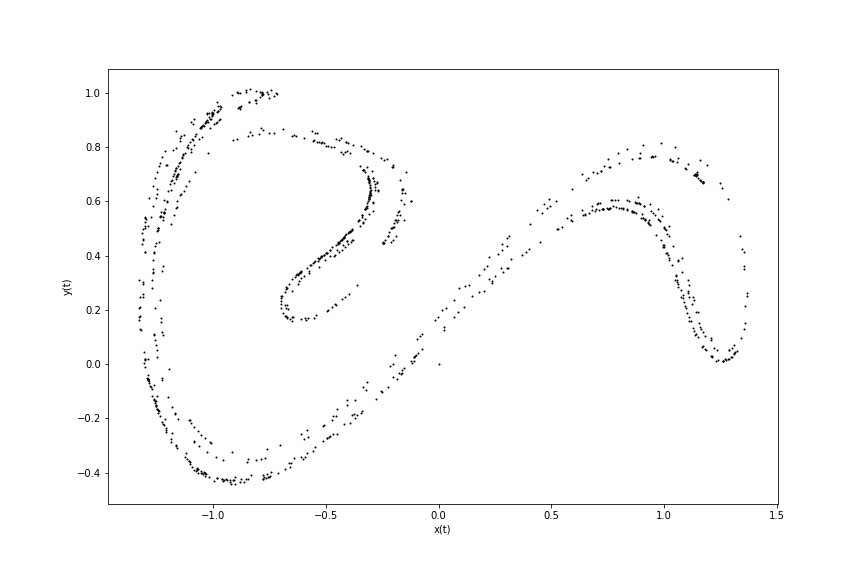
\includegraphics[width=\linewidth]{plot for driven sombrero potential equation for nu = 0.25,x_0 = 0,y_0 = 0.0,m = 1.0,omega = 1.0,F = 0.4.png}
  \caption{plot for driven sombrero potential equation for nu = 0.25,x_0 = 0,y_0 = 0.0,m = 1.0,omega = 1.0,F = 0.4.png}
  \label{fig:1}
\end{figure}



Figure \ref{fig:1} shows  a plot for driven sombrero potential equation for
nu = 0.25,x_0 = 0,y_0 = 0.0,m = 1.0,omega = 1.0,F = 0.4 \text{ or a boat.}

In total we have 8 plots/graphs for :
\text{ Plot for driven sombrero potential equation for } nu = 0.25,x_0 = -0.9,y_0 = 0.0,m = 1.0,omega = 1.0,F = 0.18
\text{ Plot for driven sombrero potential equation for }nu = 0.25,x_0 = 0,y_0 = 0.0,m = 1.0,omega = 1.0,F = 0.4
\text{ Plot for driven sombrero potential equation for }nu = 0.25,x_0 = 0.2,y_0 = 0.1,m = 1.0,omega = 1.0,F = 0.25
\text{ Plot for driven sombrero potential equation for }nu = 0.25,x_0 = 0.9,y_0 = 0.0,m = 1.0,omega = 1.0,F = 0.18
\text{ plot for driven sombrero potential equation for }nu = 0.25,x_0 = -0.9,y_0 = 0.0,m = 1.0,omega = 1.0,F = 0.18
\text{ plot for driven sombrero potential equation for }nu = 0.25,x_0 = 0,y_0 = 0.0,m = 1.0,omega = 1.0,F = 0.4
\text{ plot for driven sombrero potential equation for }nu = 0.25,x_0 = 0.2,y_0 = 0.1,m = 1.0,omega = 1.0,F = 0.25
\text{ plot for driven sombrero potential equation for }nu = 0.25,x_0 = 0.9,y_0 = 0.0,m = 1.0,omega = 1.0,F = 0.18

but for some unknown reason they dont want to show up.
\end{document}